% !TeX program = xelatex
% Compile with XeLaTeX. Keep fonts/ beside this file.
% The merged version additionally uses the original assets/ folder.
% Theme definitions and slide content are included here; no other .tex is required.
\documentclass[aspectratio=169,11pt]{beamer}
% Visual system and reusable TikZ helpers.
\usepackage{lmodern}
\usepackage{fontspec}
\usefonttheme{professionalfonts}
\setsansfont{NimbusSans-Regular.otf}[Path=fonts/,BoldFont=NimbusSans-Bold.otf,ItalicFont=NimbusSans-Italic.otf,BoldItalicFont=NimbusSans-BoldItalic.otf]
\newfontfamily\editorial{P052-Italic.otf}[Path=fonts/]
\usepackage{amsmath,amssymb,graphicx,tikz}
\usetikzlibrary{arrows.meta,calc,shapes.geometric,decorations.pathreplacing}
\setbeamertemplate{navigation symbols}{}
\setbeamertemplate{headline}{}
\setbeamertemplate{footline}{}
\setbeamertemplate{frametitle}{}
\setbeamersize{text margin left=0pt,text margin right=0pt}
\setbeamercolor{background canvas}{bg=white}
\setbeamercovered{invisible}
\definecolor{charcoal}{HTML}{17201D}
\definecolor{ivory}{HTML}{F4F0E7}
\definecolor{forest}{HTML}{245842}
\definecolor{gold}{HTML}{D9B45E}
\definecolor{goldink}{HTML}{88631D}
\definecolor{sage}{HTML}{A8C1AE}
\definecolor{muted}{HTML}{6B766D}
\definecolor{rulegray}{HTML}{D5D9CE}
\definecolor{softgreen}{HTML}{E4EADF}
\definecolor{softgold}{HTML}{EEE1BF}
\definecolor{stone}{HTML}{9DADA2}
\newcommand{\Light}{\colorlet{bg}{white}\colorlet{fg}{charcoal}\colorlet{accent}{forest}\colorlet{subtle}{muted}\colorlet{linecol}{rulegray}}
\newenvironment{canvas}{\begin{tikzpicture}[remember picture,overlay]\begin{scope}[shift={(current page.north west)},x=1cm,y=-1cm]\fill[bg] (0,0) rectangle (16,9);}{\end{scope}\end{tikzpicture}}
\hyphenpenalty=10000
\exhyphenpenalty=10000
\newcommand{\T}[6]{\pgfmathsetmacro{\leading}{#4*1.15}\node[anchor=north west,inner sep=0pt,align=left,text width=#3cm,text=#5,font=\fontsize{#4}{\leading}\selectfont] at (#1,#2) {#6};}
\newcommand{\C}[5]{\node[anchor=center,inner sep=0pt,text=#4,font=\fontsize{#3}{#3}\selectfont] at (#1,#2) {#5};}
\newcommand{\Header}[2]{\T{.8}{.52}{14}{7}{accent}{\textbf{#1}}\T{.8}{1.03}{14.4}{22}{fg}{\textbf{#2}}}
\newcommand{\Footer}[1]{\draw[linecol,line width=.35pt] (.8,8.39)--(15.2,8.39);\T{.8}{8.56}{12.9}{5.5}{subtle}{#1}\T{14.5}{8.52}{.7}{7}{subtle}{\textbf{\insertframenumber}\,/\,\inserttotalframenumber}}
\newcommand{\Play}[3]{\fill[#3] (#1,#2) circle (.20);\fill[ivory] ({#1-.055},{#2-.09})--({#1-.055},{#2+.09})--({#1+.105},#2)--cycle;}
\newcommand{\Thumb}[5]{\begin{scope}\clip (#2,#3) rectangle ({#2+#4},{#3+#5});\node[anchor=north west,inner sep=0pt] at ({#2-(#1-1)*#4},{#3-(#4-#5)/2}) {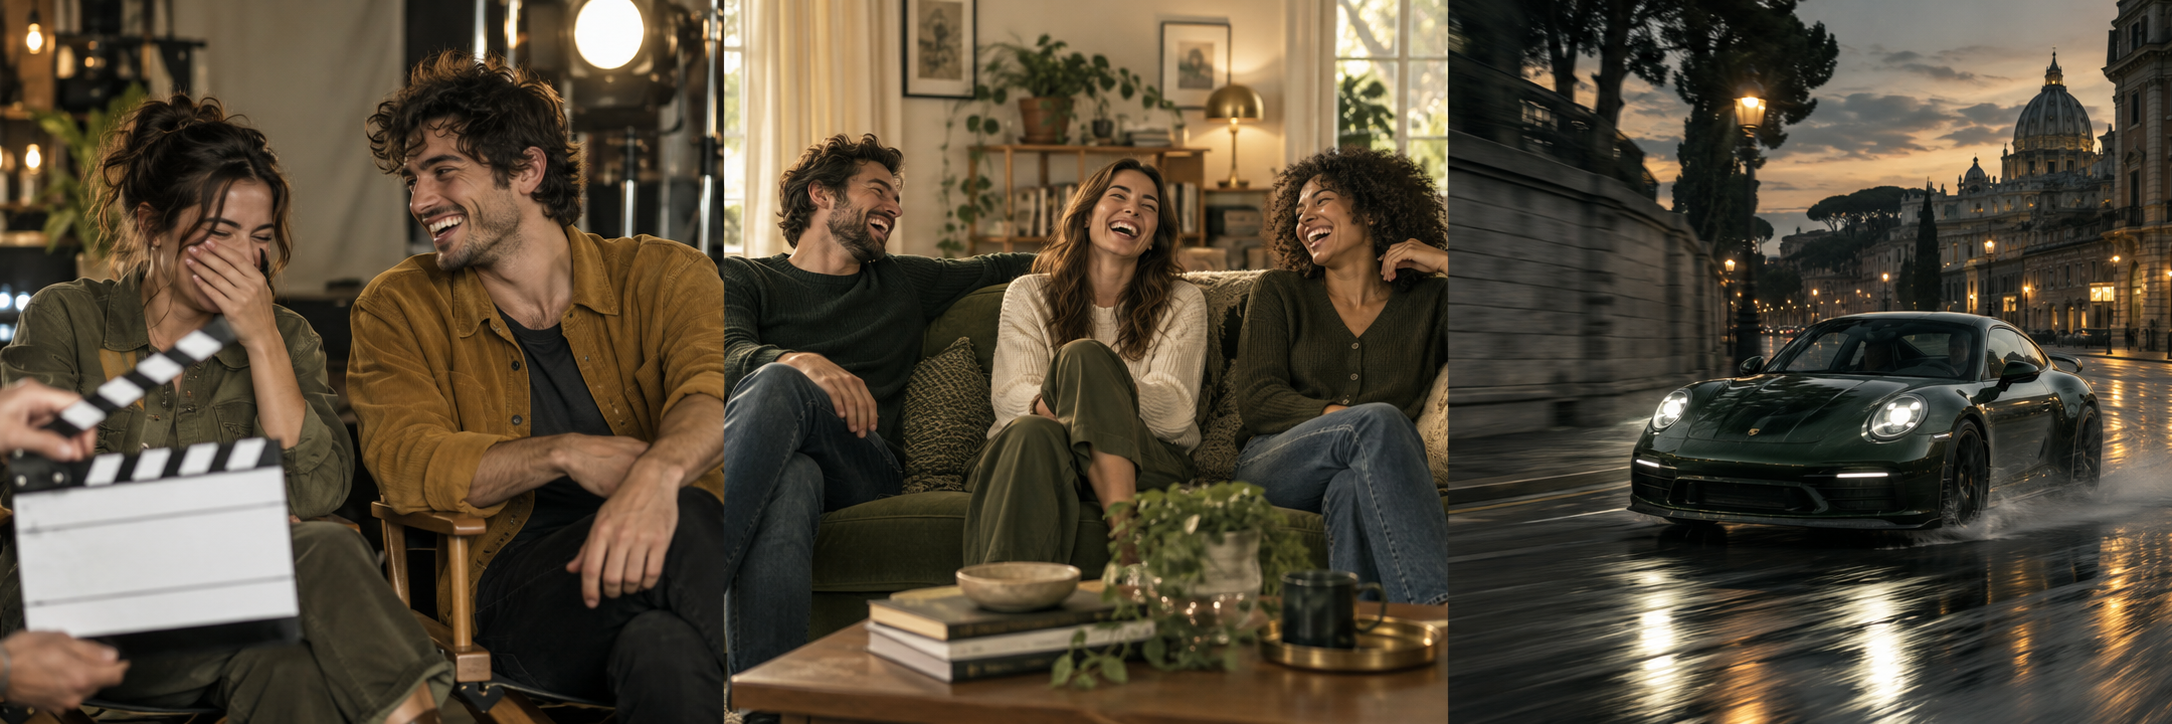
\includegraphics[width=\dimexpr#4cm*3\relax]{assets/videos.png}};\end{scope}}
\newcommand{\Force}[1]{\only<#1>{\relax}}
\title{Recommendation Algorithms: Bob's Next Video}
\author{Sami}
\date{}
\hypersetup{pdftitle={Recommendation Algorithms | Sami | Speaker 1},pdfauthor={Sami},pdfsubject={Feedback, user-item matrix, and content-based filtering},pdfpagemode=FullScreen}

% ---------- Adapter for the supplied continuation ----------
% Colors and helpers are local to each frame, so Sami's frames remain intact.
\usepackage{bm,booktabs,array,adjustbox}
\usetikzlibrary{positioning,fit,matrix,overlay-beamer-styles}
\newsavebox{\PartContent}
\newsavebox{\PartTitle}
\newcommand{\PartSectionOffset}{1}
\newcommand{\PartSectionNumber}{%
  \ifnum\numexpr\insertframenumber-\PartSectionOffset\relax<10 0\fi
  \number\numexpr\insertframenumber-\PartSectionOffset\relax}
\newcommand{\PartPalette}[1]{%
  \csname #1\endcsname
  \colorlet{ink}{fg}\colorlet{muted}{subtle}%
  \colorlet{blue}{accent}\colorlet{cyan}{accent}%
  \colorlet{teal}{forest}\colorlet{amber}{goldink}%
  \colorlet{rose}{goldink}\colorlet{violet}{forest}%
  \colorlet{paleBlue}{softgreen}\colorlet{paleTeal}{softgreen}%
  \colorlet{paleAmber}{softgold}\colorlet{paleRose}{softgold}%
  \colorlet{paleViolet}{softgreen}\colorlet{panel}{bg}%
  \color{fg}%
}
\newcommand{\PartHeader}[2]{%
  \T{.8}{.52}{14}{7}{accent}{\textbf{#1}}%
  \node[anchor=north west,inner sep=0pt,text=fg]
    at (.8,1.03) {\begin{adjustbox}{max width=14.4cm}\usebox{\PartTitle}\end{adjustbox}};%
}
\newcommand{\PartStart}[4]{%
  \PartPalette{#1}%
  \sbox{\PartTitle}{{\normalfont\sffamily\bfseries\fontsize{22}{25.3}\selectfont #3}}%
  \begin{canvas}
    \PartHeader{#2}{#3}
    \Footer{#4}
  \end{canvas}%
}
% Same bold Nimbus hierarchy as the reference; no extra font dependency.
\newcommand{\textbfPro}[1]{{\sffamily\bfseries\fontsize{12}{14}\selectfont #1}}
\newcommand{\micro}[1]{{\fontsize{8}{10}\selectfont\textcolor{subtle}{#1}}}
\newcommand{\callout}[3][]{%
  \begin{center}\begin{tikzpicture}
    \node[rectangle,draw=accent,fill=paleBlue,text=fg,line width=.7pt,
      inner xsep=10pt,inner ysep=7pt,text width=#2,align=left,
      font=\fontsize{11}{13.2}\selectfont,#1]
      {\hyphenpenalty=10000\relax#3\par};
  \end{tikzpicture}\end{center}%
}
\tikzset{
  box/.style={rectangle,rounded corners=2.2mm,draw=linecol,fill=panel,text=fg,align=center,
    inner sep=7pt,font=\fontsize{11}{13.2}\selectfont,line width=.85pt},
  boxblue/.style={box,draw=blue,fill=paleBlue},
  boxteal/.style={box,draw=teal,fill=paleTeal},
  boxamber/.style={box,draw=amber,fill=paleAmber},
  boxrose/.style={box,draw=rose,fill=paleRose},
  boxviolet/.style={box,draw=violet,fill=paleViolet},
  user/.style={circle,draw=forest,fill=forest,text=ivory,
    minimum size=7mm,inner sep=0pt,font=\fontsize{9}{10}\selectfont\bfseries,line width=.8pt},
  item/.style={circle,draw=goldink,fill=gold,text=charcoal,
    minimum size=7mm,inner sep=0pt,font=\fontsize{9}{10}\selectfont\bfseries,line width=.8pt},
  feat/.style={circle,draw=forest,fill=sage,text=charcoal,
    minimum size=7mm,inner sep=0pt,font=\fontsize{9}{10}\selectfont\bfseries,line width=.8pt},
  arr/.style={line width=1.1pt,draw=accent},
  greyarr/.style={line width=.8pt,draw=subtle},
  dashedarr/.style={line width=1.1pt,draw=rose,dashed}
}
% Place the original content between the fixed reference header and footer.
% Invisible overlay objects still reserve their space.
\newenvironment{PartBody}{%
  \begin{lrbox}{\PartContent}\begin{minipage}{14.4cm}
    \color{fg}\sffamily\fontsize{11}{13.2}\selectfont
    \setlength{\parindent}{0pt}%
}{%
  \end{minipage}\end{lrbox}%
  \begin{tikzpicture}[remember picture,overlay]
    \node[anchor=center,inner sep=0pt,text=fg]
      at ([yshift=-5.15cm]current page.north)
      {\begin{adjustbox}{max totalsize={14.4cm}{5.7cm}}\usebox{\PartContent}\end{adjustbox}};
  \end{tikzpicture}%
}

\hypersetup{pdftitle={Recommendation Algorithms},pdfauthor={Presentation team},pdfsubject={Recommendation algorithms}}
\begin{document}
% Sami: eight frames, 23 overlay pages.


% % FRAME 1 — 2 overlays — 00:00–00:18
% \begin{frame}[plain,label=bob]
% \Light
% \begin{canvas}
% \node[anchor=north west,inner sep=0pt] at (8.8,0) {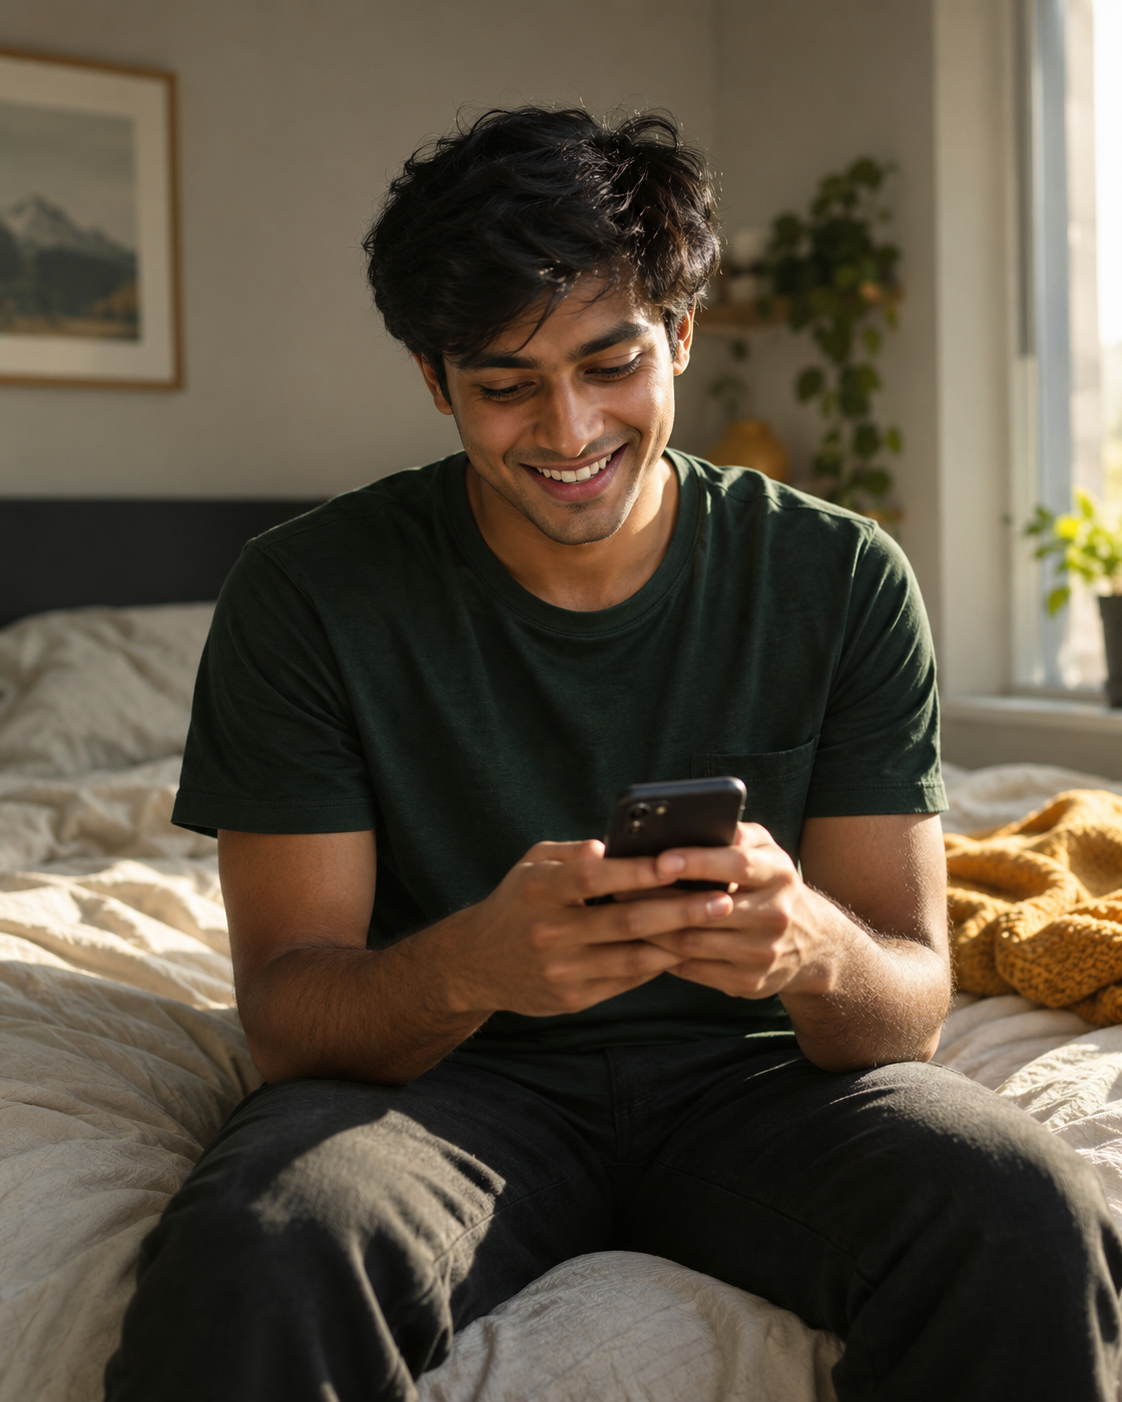
\includegraphics[width=7.2cm,height=9cm]{assets/bob.png}};
% \fill[gold] (8.68,0) rectangle (8.8,9);
% \T{.8}{.64}{7.2}{8}{goldink}{\textbf{RECOMMENDATION ALGORITHMS}}
% \T{.8}{1.55}{7.6}{39}{fg}{Your next\\{\editorial favorite.}}
% \T{.85}{4.86}{6.7}{14}{subtle}{A story about how a feed\\learns what to show you.}
% \only<2->{\draw[gold,line width=1pt] (.85,6.01)--(1.7,6.01);\T{.85}{6.3}{6.6}{24}{fg}{\textbf{Meet Bob.}}\T{.85}{7.05}{6.6}{11}{subtle}{Saturday morning. One funny video.}}
% \T{.85}{8.3}{7}{7}{subtle}{SAMI\quad /\quad DEPARTMENT OF CSE}
% \end{canvas}
% \Force{2}
% \end{frame}

% % FRAME 2 — 3 overlays — 00:18–00:40
% \begin{frame}[plain,label=feed]
% \Light
% \begin{canvas}
% \Header{01 / THE STORY}{Sunday looks familiar.}
% \T{.8}{2.45}{6.2}{17}{fg}{One video yesterday.}
% \only<2->{\T{.8}{3.35}{6}{17}{fg}{A feed full of comedy.}}
% \only<3->{\T{.8}{5.09}{6.3}{29}{forest}{\editorial Coincidence?}\T{.8}{6.48}{6.2}{14}{fg}{Something is happening\\behind the screen.}}
% % A deliberately simplified video-feed mockup, not a platform screenshot.
% \fill[charcoal,rounded corners=5mm] (8.2,2.18) rectangle (14.62,8.04);
% \fill[ivory,rounded corners=3.8mm] (8.32,2.3) rectangle (14.5,7.92);
% \fill[charcoal,rounded corners=1mm] (10.69,2.39) rectangle (12.12,2.53);
% \T{8.75}{2.85}{5.5}{10}{charcoal}{\textbf{For Bob}\hfill Sunday, 9:00 AM}
% \Thumb{1}{8.75}{3.43}{2.07}{1.25}\Play{10.54}{4.42}{forest}
% \T{11.08}{3.61}{2.9}{12}{charcoal}{\textbf{Bloopers}}\T{11.08}{4.12}{2.9}{8}{muted}{On-set laughs}
% \only<2->{\Thumb{2}{8.75}{4.91}{2.07}{1.25}\Play{10.54}{5.9}{forest}\T{11.08}{5.12}{2.9}{12}{charcoal}{\textbf{Sitcom clips}}\T{11.08}{5.63}{2.9}{8}{muted}{Best moments}
% \fill[forest] (8.75,6.41) rectangle (10.82,7.45);\draw[gold,line width=1.4pt] (9.7,6.74)--(9.7,7.12);\draw[gold,line width=.7pt] (9.55,7.12)--(9.85,7.12);\fill[gold] (9.7,6.69) circle (.105);\T{11.08}{6.61}{2.9}{12}{charcoal}{\textbf{Stand-up}}\T{11.08}{7.1}{2.9}{8}{muted}{A few more laughs}}
% \Footer{Fictional story and feed. Watch history is one of several recommendation signals. [1]}
% \end{canvas}\Force{3}
% \end{frame}

% % FRAME 3 — 3 overlays — 00:40–00:59
% \begin{frame}[plain,label=backstage]
% \Light
% \begin{canvas}
% \Header{02 / BEHIND THE SCREEN}{A ranked guess.}
% \T{.8}{2.25}{13.9}{13}{subtle}{The system uses evidence to decide what Bob might enjoy next.}
% \fill[softgreen] (.85,3.52) rectangle (4.5,5.95);
% \T{1.13}{3.91}{3.1}{18}{fg}{\textbf{Observe}}
% \T{1.13}{4.85}{3}{11}{subtle}{Watches,\\ratings, skips}
% \only<2->{\draw[-{Latex[length=3mm]},gold,line width=1.1pt] (4.72,4.72)--(5.43,4.72);\draw[goldink,line width=.8pt] (5.65,3.52) rectangle (9.64,5.95);\T{5.98}{3.91}{3.4}{18}{fg}{\textbf{Learn}}\T{5.98}{4.85}{3.3}{11}{subtle}{Build a profile.\\Score candidates.}}
% \only<3->{\draw[-{Latex[length=3mm]},gold,line width=1.1pt] (9.88,4.72)--(10.59,4.72);\T{11.05}{3.55}{3.9}{18}{goldink}{\textbf{Rank}}\foreach \y/\n/\w in {4.51/1/2.95,5.03/2/2.25,5.55/3/1.48}{\C{11.13}{\y}{10}{subtle}{\n}\fill[gold] (11.51,{\y-.12}) rectangle ({11.51+\w},{\y+.12});}\T{.85}{7.03}{14.2}{17}{fg}{That is the job of a \textbf{recommendation system}.}}
% \Footer{Simplified recommendation pipeline. Longer bars represent higher model scores. [2]}
% \end{canvas}\Force{3}
% \end{frame}

% % FRAME 4 — 3 overlays — 00:59–01:24
% \begin{frame}[plain,label=feedback]
% \Light
% \begin{canvas}
% \Header{03 / FEEDBACK}{Bob tells us in two ways.}
% \draw[rulegray] (7.9,2.53)--(7.9,6.83);
% \T{.85}{2.57}{6.4}{9}{forest}{\textbf{EXPLICIT FEEDBACK}}
% \T{.85}{3.15}{6.3}{23}{fg}{\editorial What he says.}
% \foreach \x in {1.18,2.02,2.86,3.7,4.54}{\node[star,star points=5,star point ratio=2.25,fill=goldink,minimum size=.59cm,inner sep=0pt] at (\x,4.44) {};}
% \T{.85}{5.12}{6.4}{15}{fg}{Rate. Like. Dislike.}
% \T{.85}{5.92}{6.4}{11}{muted}{A direct expression of preference.}
% \only<2->{\T{8.67}{2.57}{6.2}{9}{forest}{\textbf{IMPLICIT FEEDBACK}}\T{8.67}{3.15}{6.2}{23}{fg}{\editorial What he does.}\Play{8.96}{4.45}{forest}\draw[rulegray,line width=3.5pt] (9.44,4.45)--(14.82,4.45);\draw[forest,line width=3.5pt] (9.44,4.45)--(13.9,4.45);\fill[forest] (13.9,4.45) circle (.10);\T{8.67}{5.12}{6.4}{15}{fg}{Watch. Replay. Skip.}\T{8.67}{5.92}{6.3}{11}{muted}{Behavior that may suggest interest.}}
% \only<3->{\fill[softgold] (.85,7.12) rectangle (15.15,7.91);\T{1.12}{7.35}{13.5}{13}{charcoal}{\textbf{A long watch is a clue, not proof that Bob liked it.}}}
% \Footer{Feedback categories; behavior is ambiguous and absence of an event does not establish dislike. [3]}
% \end{canvas}\Force{3}
% \end{frame}

% % FRAME 5 — 3 overlays — 01:24–01:48
% \begin{frame}[plain,label=matrix]
% \Light
% \begin{canvas}
% \Header{04 / THE USER--ITEM MATRIX}{A few ratings. Many unknowns.}
% \T{.85}{2.25}{14.2}{11}{muted}{Rows = people. Columns = videos. Entries = ratings.}
% % Column and row headers stay stable across all overlays.
% \foreach \x/\label in {3.6/Bloopers,5.45/{Sitcom 1},7.3/Action,9.15/Travel}{\C{\x}{3.27}{11}{fg}{\label}}
% \foreach \y/\name in {4.15/Bob,5.4/Asha,6.65/Leo}{\T{.85}{\y-.16}{1.5}{13}{fg}{\textbf{\name}}}
% \foreach \row in {0,1,2}{\foreach \col in {0,1,2,3}{\pgfmathsetmacro{\xx}{2.8+1.85*\col}\pgfmathsetmacro{\yy}{3.64+1.25*\row}\fill[softgreen] (\xx,\yy) rectangle ({\xx+1.6},{\yy+1.02});}}
% \only<1>{\C{3.6}{4.15}{21}{forest}{5}\draw[-{Latex[length=2mm]},forest,line width=1pt] (1.98,4.15)--(2.61,4.15);\T{11.1}{3.92}{3.85}{16}{forest}{Bob rated\\bloopers \textbf{5}.}}
% \only<2->{\foreach \x/\y/\v in {3.6/4.15/5,5.45/4.15/4,3.6/5.4/4,7.3/5.4/2,7.3/6.65/5}{\C{\x}{\y}{21}{forest}{\v}}\foreach \x/\y in {7.3/4.15,9.15/4.15,5.45/5.4,9.15/5.4,3.6/6.65,5.45/6.65,9.15/6.65}{\C{\x}{\y}{21}{muted}{?}}\T{11.1}{3.92}{3.85}{16}{fg}{Most ratings\\are missing.}}
% \only<3->{\draw[goldink,line width=1.5pt] (6.5,3.64) rectangle (8.1,4.66);\T{11.1}{5.74}{3.85}{18}{forest}{\textbf{Unknown}\\$\boldsymbol{\ne}$ disliked.}\T{.85}{7.58}{14.3}{13}{fg}{The challenge: score a video Bob has never rated.}}
% \Footer{Illustrative explicit ratings on a 1--5 scale. A question mark means no observed rating. [3]}
% \end{canvas}\Force{3}
% \end{frame}

% % FRAME 6 — 3 overlays — 01:48–02:16
% \begin{frame}[plain,label=features]
% \Light
% \begin{canvas}
% \Header{05 / CONTENT-BASED FILTERING}{Describe videos. Learn Bob's taste.}
% \T{.85}{2.21}{13.9}{12}{subtle}{Recommend videos whose features resemble what Bob already enjoys.}
% \T{.85}{3.04}{4.2}{8}{goldink}{\textbf{VIDEOS BOB ENJOYS}}
% \Thumb{1}{.85}{3.57}{3.32}{2.38}\Play{3.82}{5.6}{forest}
% \T{.85}{6.18}{3.9}{13}{fg}{Movie bloopers}
% \only<2->{\draw[-{Latex[length=2.8mm]},gold,line width=1.1pt] (4.38,4.73)--(5.14,4.73);\T{5.48}{3.04}{3.9}{8}{goldink}{\textbf{ITEM FEATURES}}\T{5.48}{3.76}{3.5}{18}{fg}{Comedy}\T{5.48}{4.38}{3.5}{11}{subtle}{Genre, tone, topic,\\cast, duration\ldots}\draw[linecol] (5.48,5.58)--(8.7,5.58);\T{5.48}{5.94}{3.5}{11}{subtle}{Describes the video.}}
% \only<3->{\draw[-{Latex[length=2.8mm]},gold,line width=1.1pt] (9.09,4.73)--(9.83,4.73);\fill[softgreen] (10.15,3.39) rectangle (15.15,6.96);\T{10.49}{3.76}{4.25}{8}{goldink}{\textbf{BOB'S CONTENT PROFILE}}\T{10.49}{4.44}{4.25}{23}{fg}{$\mathbf p=(3,\,1)$}\T{10.49}{5.44}{4.15}{10}{fg}{Comedy: 3\quad Action: 1}\T{10.49}{6.08}{4.16}{10}{subtle}{From his feedback\\and video features.}\T{.85}{7.51}{14.3}{13}{fg}{A profile of \textbf{features}, built from a history of \textbf{feedback}.}}
% \Footer{Illustrative profile and feature strengths. Content-based filtering uses this user's history and item features. [4]}
% \end{canvas}\Force{3}
% \end{frame}

% % FRAME 7 — 4 overlays — 02:16–02:44
% \begin{frame}[plain,label=similarity]
% \Light
% \begin{canvas}
% \Header{06 / SIMILARITY}{The closer direction wins.}
% \T{.85}{2.2}{14}{11}{muted}{Compare Bob's profile with candidate video features using cosine similarity.}
% % Left: exact feature geometry. Axes use common linear scale .8 cm/unit.
% \draw[-{Latex[length=2.1mm]},muted,line width=.7pt] (1.44,6.9)--(6.1,6.9);
% \draw[-{Latex[length=2.1mm]},muted,line width=.7pt] (1.44,6.9)--(1.44,3.07);
% \T{4.74}{7.16}{2.2}{10}{muted}{Comedy}
% \T{.85}{2.76}{2}{10}{muted}{Action}
% \draw[-{Latex[length=2.8mm]},forest,line width=1.6pt] (1.44,6.9)--(3.84,6.1);
% \T{3.53}{5.46}{3}{12}{forest}{\textbf{Bob $(3,1)$}}
% % Right: two video candidates, feature values aren't ratings.
% \T{7.64}{2.89}{7.47}{8}{forest}{\textbf{CANDIDATE VIDEO FEATURES: (COMEDY, ACTION)}}
% \Thumb{2}{7.64}{3.44}{1.76}{1.06}\T{9.68}{3.49}{3.87}{12}{fg}{\textbf{A / Sitcom 2}}\T{9.68}{3.99}{3.87}{10}{muted}{$\mathbf a=(4,0)$}
% \Thumb{3}{7.64}{4.82}{1.76}{1.06}\T{9.68}{4.87}{3.87}{12}{fg}{\textbf{B / Action trailer}}\T{9.68}{5.37}{3.87}{10}{muted}{$\mathbf b=(1,4)$}
% \only<2->{\draw[-{Latex[length=2.8mm]},goldink,line width=1.6pt] (1.44,6.9)--(4.64,6.9);\T{4.83}{6.44}{1.9}{12}{goldink}{\textbf{A}}\draw[goldink,line width=.8pt] (2.35,6.9) arc[start angle=0,end angle=-18.435,radius=.91];\C{2.62}{6.66}{8}{goldink}{$\theta_A$}\T{14.03}{3.67}{1.2}{17}{goldink}{\textbf{0.95}}}
% \only<3->{\draw[-{Latex[length=2.8mm]},muted,line width=1.3pt] (1.44,6.9)--(2.24,3.7);\T{2.43}{3.54}{1.3}{12}{muted}{\textbf{B}}\draw[muted,densely dashed,line width=.7pt] (3.006,6.378) arc[start angle=-18.435,end angle=-75.964,radius=1.65];\C{2.95}{5.51}{8}{muted}{$\theta_B$}\T{14.03}{5.05}{1.2}{17}{muted}{\textbf{0.54}}}
% \only<4->{\T{7.64}{6.14}{7.5}{14}{forest}{$\displaystyle \mathrm{sim}(\mathbf p,\mathbf v)=\frac{\mathbf p\cdot\mathbf v}{\|\mathbf p\|\,\|\mathbf v\|}$}\fill[softgold] (7.64,7.51) rectangle (15.15,8.13);\T{7.87}{7.71}{7.0}{11}{charcoal}{$0.95 > 0.54$\qquad \textbf{Recommend A.}}}
% \Footer{Toy feature vectors, not star ratings. Calculated cosine scores: A = 0.9487; B = 0.5369. [4,5]}
% \end{canvas}\Force{4}
% \end{frame}

% % FRAME 8 — 2 overlays — 02:44–03:00
% \begin{frame}[plain,label=handoff]
% \Light
% \begin{canvas}
% \T{.85}{.6}{14.2}{8}{goldink}{\textbf{07 / THE NEXT QUESTION}}
% \T{.85}{1.48}{13.8}{31}{fg}{Can Bob discover\\{\editorial something different?}}
% \T{.85}{4.02}{13.4}{12}{subtle}{Familiar features can mean more of the same.}
% \draw[gold,line width=1.5pt] (.88,5.01)--(.88,6.42);
% \T{1.2}{5.01}{13.3}{19}{fg}{What if people with Bob's taste love\\a video with completely different tags?}
% \only<2->{\T{.85}{7.05}{12.8}{25}{goldink}{\textbf{Collaborative filtering}}\draw[-{Latex[length=4mm]},gold,line width=1.3pt] (13.23,7.45)--(15.03,7.45);\T{.88}{8.05}{13.3}{8}{subtle}{My teammate takes the story from here.}}
% \end{canvas}\Force{2}
% \end{frame}

% Continuation frame 1: original text and reveals retained.
\begin{frame}[plain]
\PartStart{Light}{\PartSectionNumber\ / COLLABORATIVE FILTERING}{Collaborative filtering}{2305033 - collaborative}
\begin{PartBody}
\centering
\begin{tikzpicture}
\node[user] (u1) at (2,3.8) {U1}; \node[user] (u2) at (2,2.75) {U2}; \node[user] (u3) at (2,1.7) {U3}; \node[user] (u4) at (2,.65) {U4};
\node[item] (m1) at (7,4.15) {M1}; \node[item] (m2) at (7,3.1) {M2}; \node[item] (m3) at (7,2.05) {M3}; \node[item] (m4) at (7,1.0) {M4};
\draw[greyarr,visible on=<1->] (u1)--(m1); \draw[greyarr,visible on=<1->] (u1)--(m2); \draw[greyarr,visible on=<1->] (u2)--(m3); \draw[greyarr,visible on=<1->] (u2)--(m1); \draw[greyarr,visible on=<1->] (u2)--(m2); \draw[greyarr,visible on=<1->] (u3)--(m3); \draw[greyarr,visible on=<1->] (u4)--(m4);
\draw[dashedarr,visible on=<2->] (u1)--node[above,sloped,font=\scriptsize,text=rose]{predict}(m3);
\node[boxteal,text width=4.1cm,visible on=<3->] at (11.2,2.4) {\textbfPro{Collaborative signal}\\If users with similar histories liked $M_3$, estimate that $U_1$ may also like $M_3$.};
\end{tikzpicture}
\end{PartBody}
\end{frame}

% Continuation frame 2: original text and reveals retained.
\begin{frame}[plain]
\PartStart{Light}{\PartSectionNumber\ / TWO FAMILIES}{Collaborative filtering has two main families}{2305033 - two families}
\begin{PartBody}
\centering
\begin{tikzpicture}[outer sep=0pt]
\node[boxteal,text width=5.8cm,visible on=<1->] (r) at (6.7,5.3) {\textbfPro{Shared evidence}\\sparse user--item matrix $R$};
\node[boxblue,text width=5.4cm,minimum height=3.0cm,visible on=<2->] (mem) at (3.25,2.35) {\textbfPro{Memory-based}\\[3pt]Use $R$ directly\\Find similar users or items\\Predict from neighbours\\[3pt]\micro{User-KNN \textbullet\ Item-KNN}};
\node[boxviolet,text width=5.4cm,minimum height=3.0cm,visible on=<3->] (model) at (10.15,2.35) {\textbfPro{Model-based}\\[3pt]Learn parameters from $R$\\Compress users and items\\Predict from learned vectors\\[3pt]\micro{Matrix factorization \textbullet\ SVD}};
\draw[arr,visible on=<2->] ($(r.south west)!0.2!(r.south east)$)--(mem.north);
\draw[arr,visible on=<3->] ($(r.south west)!0.8!(r.south east)$)--(model.north);
\node[boxamber,text width=12.6cm,visible on=<4->] at (6.7,0.0) {\textbfPro{Same evidence:} neighbours now, or learned structure first.};
\end{tikzpicture}
\end{PartBody}
\end{frame}

% Continuation frame 3: original text and reveals retained.
\begin{frame}[plain]
\PartStart{Light}{\PartSectionNumber\ / MEMORY-BASED METHODS}{Memory-based methods}{2305033 - memory based}
\begin{PartBody}
\centering
\begin{tikzpicture}
\node[user] (target) at (6,2.7) {U};
\foreach \x/\y/\n in {4.3/3.9/A,4.8/1.55/B,7.25/3.6/C,7.8/1.6/D,5.9/4.2/E}{\node[user] (u\n) at (\x,\y) {\n};}
\draw[dashedarr,visible on=<2->] (target)--(uA); \draw[dashedarr,visible on=<2->] (target)--(uB);
\draw[greyarr,visible on=<3->] (uA)--(8.15,2.56); \draw[greyarr,visible on=<3->] (uB)--(8.15,2.56);
\node[item,visible on=<3->] (m) at (8.15,2.56) {M};
\node[boxblue,text width=3cm,visible on=<1->] at (1.6,2.55) {\textbfPro{User-based}\\find users similar to target user};
\node[boxteal,text width=3cm,visible on=<1->] at (10.8,3.25) {\textbfPro{Item-based}\\find items similar to target item};
\node[boxteal,text=ink,line width=.7pt,anchor=north,text width=12cm,visible on=<4->] at (6.5,.9) {Prediction comes from observed neighbours, without first learning a latent representation.};
\end{tikzpicture}
\end{PartBody}
\end{frame}

% Continuation frame 4: original text and reveals retained.
\begin{frame}[plain]
\PartStart{Light}{\PartSectionNumber\ / LIMITATIONS}{Why memory-based methods struggle at scale}{2305033 - limitations}
\begin{PartBody}
\centering
\begin{tikzpicture}[node distance=.75cm]
\node[boxrose,text width=2.9cm,visible on=<1->] (s) {\textbfPro{Sparsity}\\two users may overlap on very few items};
\node[boxamber,text width=3.2cm,right=of s,visible on=<2->] (scale) {\textbfPro{Scalability}\\similarity over millions of users/items is expensive};
\node[boxviolet,text width=3.2cm,right=of scale,visible on=<3->] (partial) {\textbfPro{Preference is partial}\\a click does not always mean preference};
\node[boxteal,text width=4.6cm,below=1.1cm of scale,visible on=<4->] (sol) {\textbfPro{Model-based direction}\\Learn a compact model once, then reuse it for prediction.};
\draw[arr,visible on=<4->] (s)--(sol); \draw[arr,visible on=<4->] (scale)--(sol); \draw[arr,visible on=<4->] (partial)--(sol);
\end{tikzpicture}
\end{PartBody}
\end{frame}

% Continuation frame 5: original text and reveals retained.
% \begin{frame}[plain]
% \PartStart{Light}{\PartSectionNumber\ / MATRIX FORMULATION}{Model-based matrix formulation}{2305033 - model formulation}
% \begin{PartBody}
% \centering
% \begin{tikzpicture}
% \node[boxrose,inner sep=6pt,visible on=<1->] (r) at (2.4,2.75) {\begin{tabular}{ccccc}5&?&4&?&1\\?&4&?&5&?\\4&?&?&4&2\\?&1&2&?&4\\5&?&?&?&4\end{tabular}};
% \node[font=\LARGE\bfseries,text=blue,visible on=<2->] at (5.0,2.75) {$\approx$};
% \node[boxblue,inner sep=6pt,visible on=<2->] (p) at (7.1,2.75) {\begin{tabular}{ccc}.6&.1&.8\\.7&.2&.7\\.1&.9&.9\\.9&.1&.1\\.2&.7&.8\end{tabular}};
% \node[font=\LARGE\bfseries,text=blue,visible on=<2->] at (8.9,2.75) {$\times$};
% \node[boxteal,inner sep=6pt,visible on=<2->] (q) at (11.4,2.75) {\begin{tabular}{ccccc}.9&.5&.7&.8&.2\\.1&.8&.2&.9&.3\\.5&.1&.8&.9&.3\end{tabular}};
% \node[boxteal,text=ink,line width=.7pt,anchor=north,text width=11.8cm,visible on=<3->] at (7,1.15) {Learn $P$ and $Q$ so that $p_u^\top q_i$ matches known values in $R$ and predicts the missing ones.};
% \end{tikzpicture}
% \end{PartBody}
% \end{frame}

% Continuation frame 6: original text and reveals retained.
\begin{frame}[plain]
\PartStart{Light}{\PartSectionNumber\ / LATENT FEATURES}{Model-based latent features}{2305033 - model representation}
\begin{PartBody}
\centering
\begin{tikzpicture}
\node[boxrose,text width=2.0cm,visible on=<1->] (r) at (1.6,3.1) {\textbfPro{Large sparse matrix}\\$m\times n$\\mostly unknown};
\node[boxblue,text width=2.0cm,visible on=<2->] (p) at (5.1,3.1) {\textbfPro{User matrix}\\$P$\\$m\times k$};
\node[boxteal,text width=2.0cm,visible on=<2->] (q) at (8.4,3.1) {\textbfPro{Item matrix}\\$Q^\top$\\$k\times n$};
\draw[arr,visible on=<2->] (r)--(p); \draw[arr,visible on=<2->] (p)--(q);
\node[boxamber,text width=3.2cm,visible on=<3->] at (11.8,2.7) {{\editorial\fontsize{14}{16}\selectfont Why possible?}\\User preferences are not random; they contain reusable patterns.};
\node[boxteal,text=ink,line width=.7pt,anchor=north,text width=10.8cm,visible on=<4->] at (6.5,.55) {The model may discover axes such as ``mainstream vs niche'' or ``light comedy vs dark drama'' without human labels.};
\end{tikzpicture}
\end{PartBody}
\end{frame}

% Transition from the methodology to the implementation algorithms.
\begin{frame}[plain]
\PartStart{Light}{\PartSectionNumber\ / FROM METHOD TO ALGORITHM}{How do these methods work in practice?}{2305033 $\rightarrow$ 2305052}
\begin{PartBody}
\centering
\begin{tikzpicture}
\node[boxteal,text width=10.8cm,minimum height=1.25cm,visible on=<1->] (method) at (6.5,4.05)
  {{\editorial\fontsize{15}{17}\selectfont We have seen the methodology}\\[3pt]
   Collaborative evidence can be used directly or compressed into latent factors.};
% \node[font=\fontsize{15}{17}\selectfont\bfseries,text=accent,text width=13.2cm,align=center,visible on=<2->] at (6.5,2.72)
%   {But how do these ideas become working algorithms?};
\node[boxblue,text width=4.1cm,minimum height=1.25cm,visible on=<2->] (knn) at (2.85,1.35)
  {\textbfPro{KNN}\\Memory-based prediction};
\node[boxamber,text width=4.1cm,minimum height=1.25cm,visible on=<3->] (svd) at (9.85,1.50)
  {\textbfPro{SVD}\\Model-based prediction};
\draw[arr,-{Latex[length=2.8mm]},visible on=<2->] (6.35,2.97) -- (knn.north east);
\draw[arr,-{Latex[length=2.8mm]},visible on=<3->] (6.35,2.97) -- (svd.north west);
\end{tikzpicture}
\end{PartBody}
\end{frame}

% Continuation: the next presenter begins with KNN.
\begin{frame}[plain]
\PartStart{Light}{\PartSectionNumber\ / NEAREST NEIGHBOURS}{KNN predicts from nearest neighbours}{2305052 - KNN}
\begin{PartBody}
\begin{columns}[T,onlytextwidth]
\column{.45\textwidth}
\centering
\begin{tikzpicture}[scale=.93]
\node[user] (t) at (2.3,2.6) {T};
\node[user] (a) at (1.2,3.6) {A}; \node[user] (b) at (3.6,3.35) {B}; \node[user] (c) at (1.0,1.7) {C}; \node[user] (d) at (3.7,1.35) {D};
\draw[dashedarr,visible on=<2->] (t)--(a); \draw[dashedarr,visible on=<2->] (t)--(b); \draw[dashedarr,visible on=<2->] (t)--(c);
\node[boxviolet,visible on=<2->] at (2.35,.35) {$k=3$ neighbors};
\end{tikzpicture}
\column{.55\textwidth}
\visible<3->{\callout[draw=violet!55,fill=paleViolet,align=center]{6.5cm}{\textbfPro{Weighted prediction}\\[3pt]$\displaystyle \hat r_{ui}=\bar r_u+\frac{\sum_{v\in N(u)}s(u,v)(r_{vi}-\bar r_v)}{\sum_{v\in N(u)} |s(u,v)|}$}}
\vspace{.15cm}
\visible<4->{\small The neighborhood provides local evidence, usually measured by cosine or Pearson similarity.}
\end{columns}
\end{PartBody}
\end{frame}

% The cosine-similarity recap was removed because it was already introduced earlier.
% The next presenter continues with the model-based algorithm.
\begin{frame}[plain]
\PartStart{Light}{\PartSectionNumber\ / LATENT FACTORS}{SVD learns latent factors}{2305052 - SVD}
\begin{PartBody}
\centering
\begin{tikzpicture}
\node[boxrose,text width=2.0cm,visible on=<1->] at (0.3,3.15) {\textbfPro{Observed}\\$R$\\$m\times n$};
\node[font=\LARGE\bfseries,text=blue,visible on=<2->] at (2.15,3.15) {$\approx$};
\node[boxblue,text width=1.5cm,visible on=<2->] at (3.75,3.15) {$U_k$\\$m\times k$};
\node[boxamber,text width=1.5cm,visible on=<2->] at (5.98,3.15) {$\Sigma_k$\\$k\times k$};
\node[boxteal,text width=1.5cm,visible on=<2->] at (8.15,3.15) {$V_k^\top$\\$k\times n$};
\node[boxviolet,text width=2.15cm,visible on=<3->] at (10.79,3.15) {\textbfPro{Prediction}\\$\hat r_{ui}=p_u^\top q_i$};
\node[boxviolet,text=ink,line width=.7pt,anchor=north,text width=10.4cm,visible on=<4->] at (6.4,1.48) {$\displaystyle \min_{P,Q}\sum_{(u,i)\in\Omega}(r_{ui}-p_u^\top q_i)^2+\lambda(\lVert p_u\rVert^2+\lVert q_i\rVert^2)$};

\end{tikzpicture}
\end{PartBody}
\end{frame}

% Continuation frame 10: original text and reveals retained.
\begin{frame}[plain]
\PartStart{Light}{\PartSectionNumber\ / RECOMMENDER WORKFLOW}{End-to-end recommender workflow}{2305052 - workflow}
\begin{PartBody}
\centering
\begin{tikzpicture}
\node[boxblue,visible on=<1->] (a) at (0.5,3.25) {Sparse data};
\node[boxteal,visible on=<2->] (b) at (2.98,3.25) {Train\\\micro{SGD / ALS}};
\node[boxamber,visible on=<3->] (c) at (5.69,3.25) {Latent vectors\\$P,Q$};
\node[boxviolet,visible on=<4->] (d) at (8.39,3.25) {Predict\\$\hat r_{ui}$};
\node[boxrose,visible on=<5->] (e) at (10.33,3.25) {Rank\\top-$N$};
\draw[arr,visible on=<2->] (a)--(b); \draw[arr,visible on=<3->] (b)--(c); \draw[arr,visible on=<4->] (c)--(d); \draw[arr,visible on=<5->] (d)--(e);
\node[boxblue,text width=2.75cm,visible on=<6->] at (0.75,1.25) {\textbfPro{KNN}\\Explainable, weaker at scale};
\node[boxteal,text width=2.75cm,visible on=<7->] at (5.12,1.25) {\textbfPro{MF / SVD}\\Compressed latent factors};
\node[boxviolet,text width=3.05cm,visible on=<8->] at (9.5,1.25) {\textbfPro{Modern systems}\\Hybrid: content + collaborative};
\end{tikzpicture}
\end{PartBody}
\end{frame}

% Continuation frame 11: original text and reveals retained.
\begin{frame}[plain]
\PartStart{Light}{\PartSectionNumber\ / TAKEAWAYS}{Takeaways}{Conclusion}
\begin{PartBody}
\centering
\begin{tikzpicture}
\node[box,draw=forest,fill=softgreen,text=charcoal,text width=2.65cm,visible on=<1->] (a) at (0.45,2.7) {\textbfPro{Sparse matrix}\\Observed only partially.};
\node[box,draw=forest,fill=softgreen,text=charcoal,text width=2.65cm,visible on=<2->] (b) at (4.10,2.7) {\textbfPro{Two families}\\Content + collaborative.};
\node[box,draw=forest,fill=softgreen,text=charcoal,text width=2.65cm,visible on=<3->] (c) at (7.65,2.7) {\textbfPro{Scaling idea}\\Compress into latent factors.};
\node[box,draw=forest,fill=softgreen,text=charcoal,text width=2.65cm,visible on=<4->] (d) at (11.17,2.7) {\textbfPro{Final output}\\Ranked personalized choices.};
\end{tikzpicture}
\vspace{.35cm}
\visible<5->{\callout[rounded corners=2.2mm,draw=goldink,fill=softgold,text=charcoal]{11.6cm}{\textbfPro{The system does not know exactly what we will like \\ it estimates from patterns shared across users, items and context.}\par\vspace{2pt}}}
\end{PartBody}
\end{frame}

\end{document}
